\section{System design}
This section depicts and elaborates on the solar panel drive's final hardware design. Design choices made within the circuit and mechanical design are explained. Further, the reasons for deployed redundancy, fault tolerance, and simplifications are given.

\subsection{Circuit design}
\autoref{fig:circuit_schematic} displays the complete circuit setup.
Since no single failure in any of the system's components shall compromise the operation of the solar panel drive, redundancy is applied for the microcontroller, actuator, and sensors. Thus, the setup integrated two Arduino Mega 2560. They function in a watchdog configuration, where the second microcontroller -- the slave -- is in hot standby and ready to take over. Both microcontrollers can command and receive feedback from the actuators and sensors. The Arduinos communicate with each other through their communication pins, shown in the orange and yellow wires from TX2/RX2 to RX3/TX3 in \autoref{fig:circuit_schematic}. 

This design includes two stepper motors. When stepper motor 1 is operative, stepper motor 2 is in stand by and ready to take over. The state of each of the stepper motors is indicated through four LEDs -- two red and two green. A constant green light indicates that the motor is in stand by and ready to receive commands, while a red light lets the user know that the respective motor is out of service and not operational. When a motor receives a command and rotates, both green and red LEDs are turned on. Likewise, the LCD prints which motor is active and its current angle. The LEDs and the LCD are solely connected to the master microcontroller. Although connecting the visual feedback components to the slave Arduino is simple, the experimental setup does not include this setup since there are limited jumper wires available. The code for the slave microcontroller, shown in appendix \ref{appendix:slave}, includes the functionality of the LEDs and LCD. The stepper motors connect to their respective driver boards and are powered through the 5V pin of the master Arduino. Redundancy is not applied for the powering of the motors. An external power source could be used, but for simplification reasons of the experimental setup, the Arduino is considered to be sufficient.

\begin{figure}[H]
    \centering
   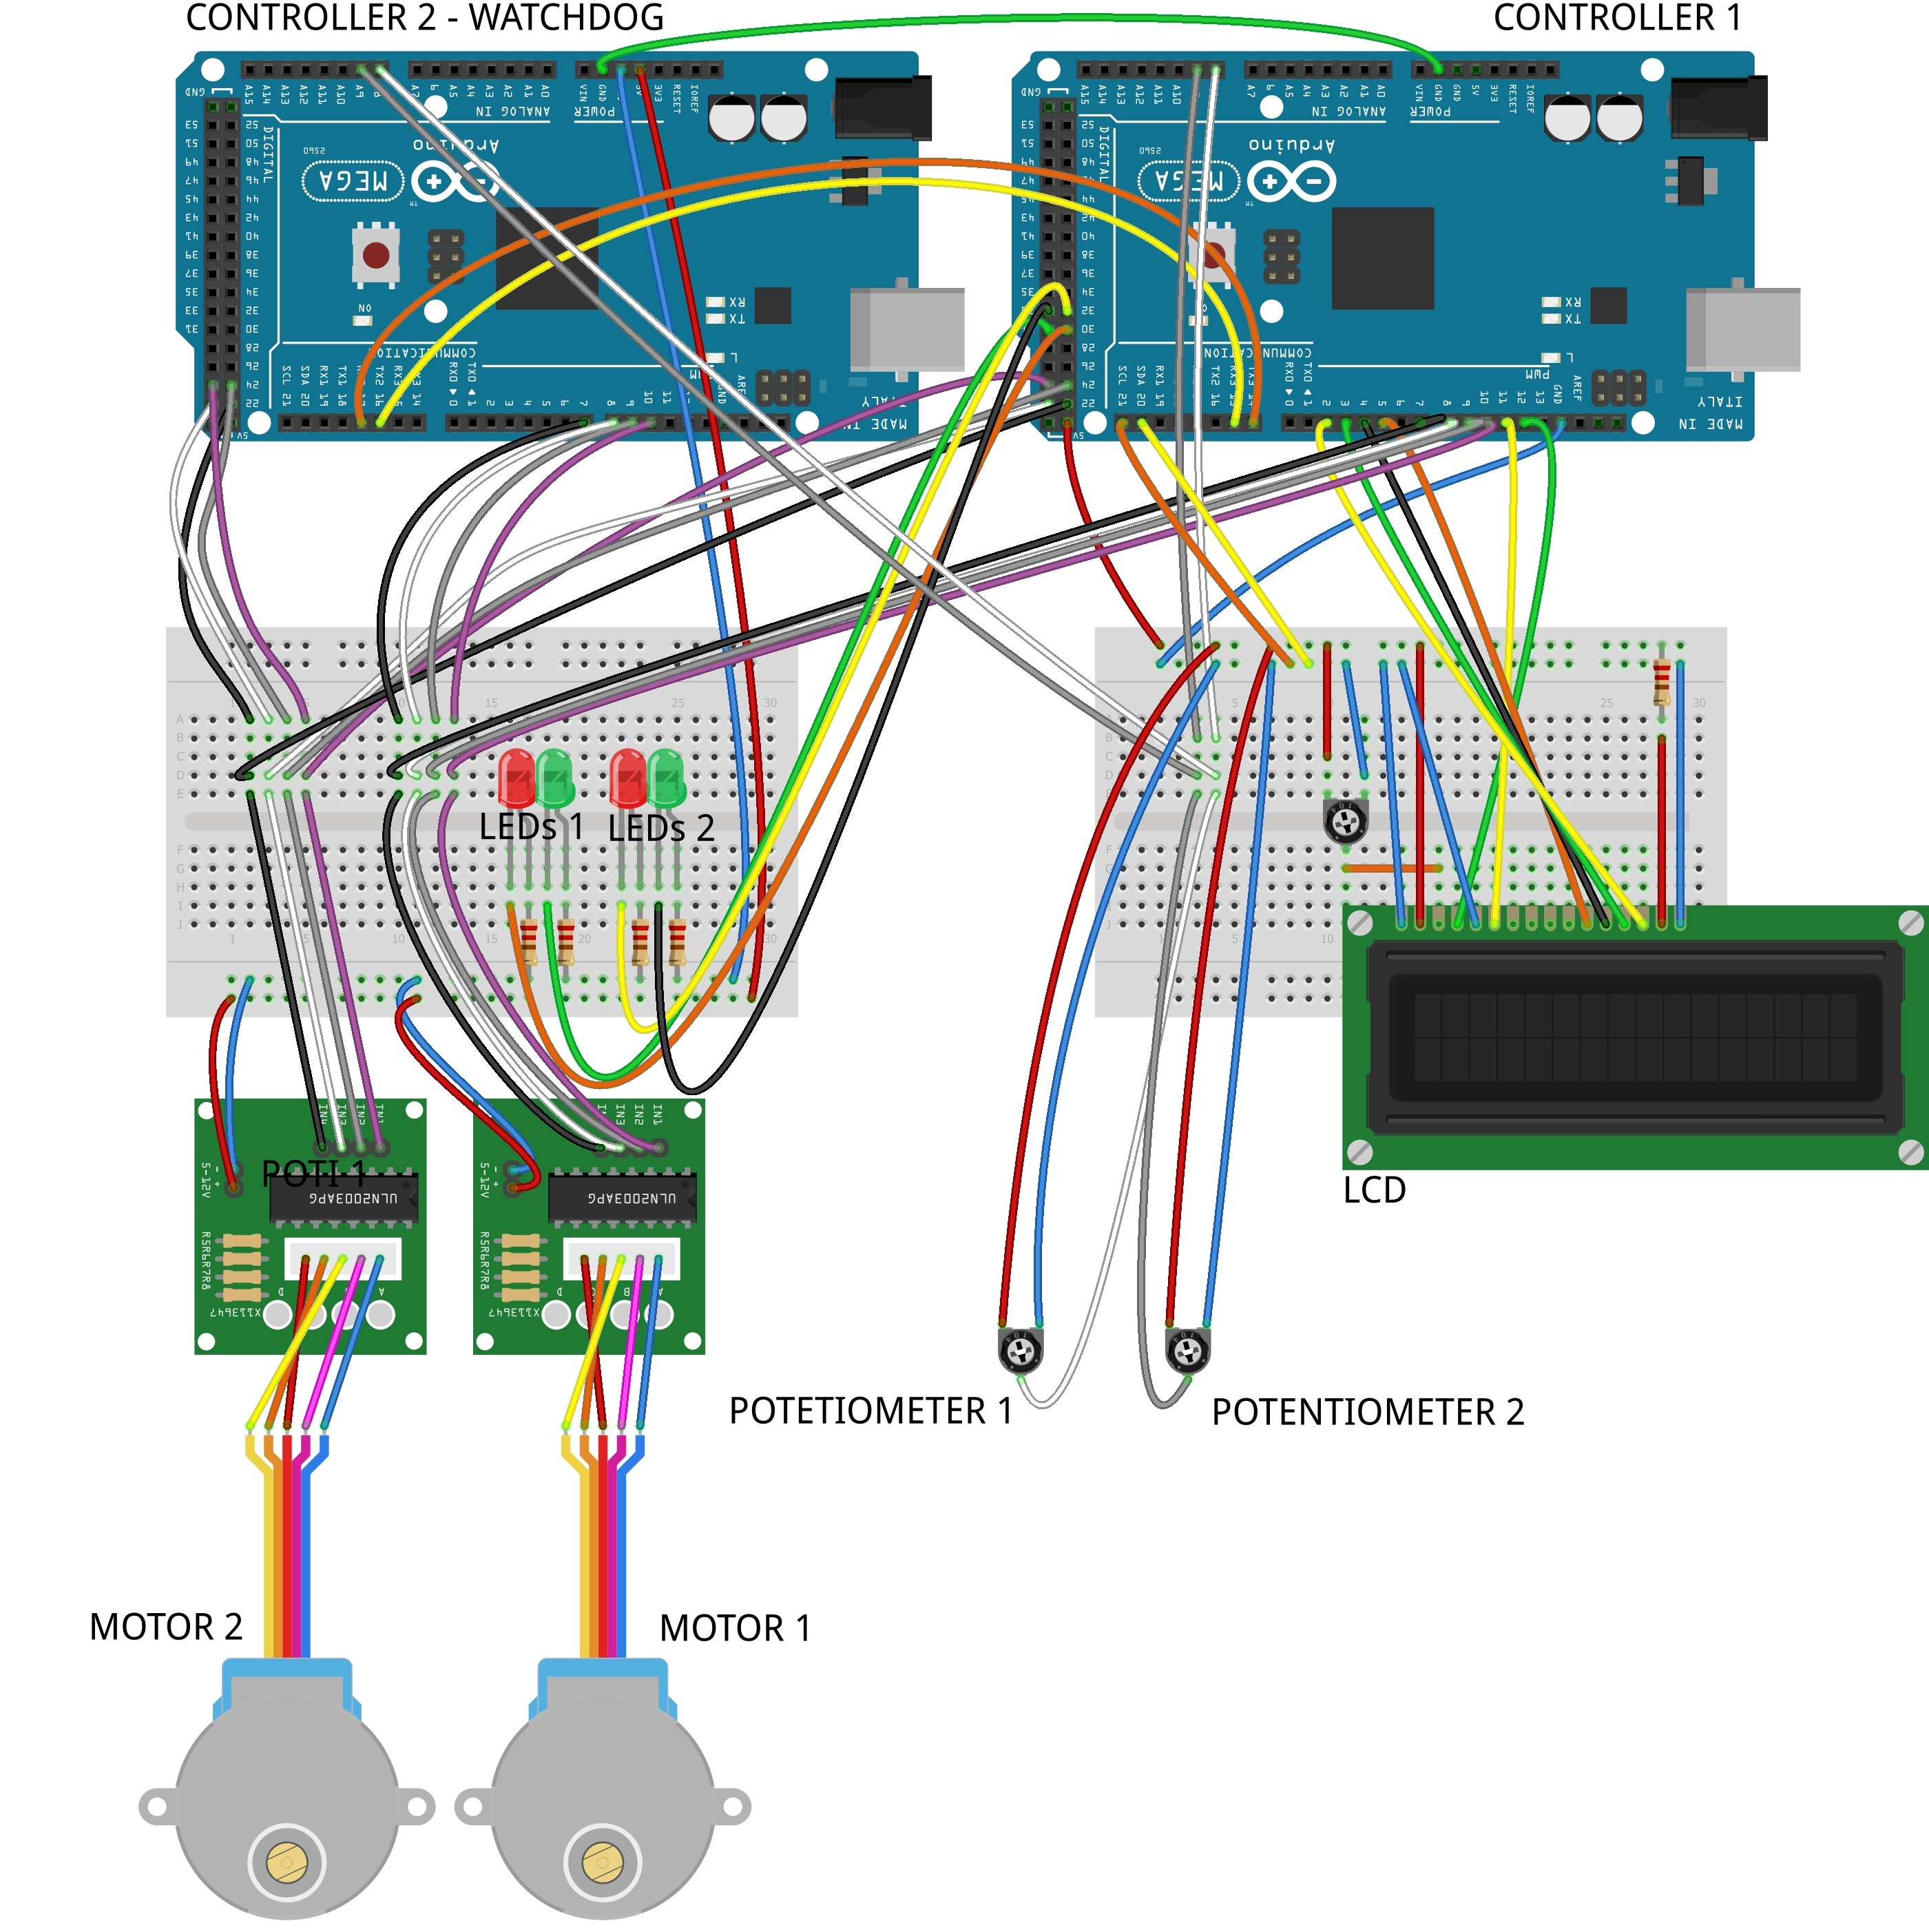
\includegraphics[width=0.7\textwidth]{figures/circuit.jpg}
    \caption{Circuit schematic}
     \label{fig:circuit_schematic}
\end{figure}

As explained in \autoref{sec:preliminary_analysis}, verification of the angle is necessary since the stepper motor alone does not return adequate feedback about its position.  Here, potentiometers are used to detect the angular position of the solar panel and verify if the assigned angle is reached. To verify the functionality of the system sufficiently, a pair of potentiometers receives the motor's rotation through the connected axis, compare \autoref{fig:mech_design}, and votes on the status of the system. The experimental setup only uses two potentiometers instead of the needed four to also receive feedback on the second stepper motor's position. The complete setup is considered to be analog to the first stepper motor's configuration and executed from the experimental design but implemented into the software architecture. The potentiometers sit close to each other and are powered, likewise to the motors, through the Arduino board.

Further, the system possesses two buttons represented by two cables that connect to pin 20 and 21 of the Arduino master board. The former is forcing the system into its safe mode - meaning the solar panel is rotated to a predefined safe angle. The latter is initiating a reset frequency, after which normal operation can be continued.

\subsection{Mechanical design}
\autoref{fig:mech_design} shows the mechanical set-up of the solar panel drive mechanism. On the left side, the stepper motors are attached to the wooden stand representing the mounting structure. Opposite, the redundant potentiometer pair is embedded into the stand and connected through a wooden axis to stepper motor 1. The mock-up solar panel is fixed to the wooden axis. Thus, the rotation of the stepper motor is conveyed to the potentiometers, while the solar panel moves according to the user's input. Theoretically, once the second stepper motor takes over, it must be able to drive the solar panel. Due to the mechanical complexity of this configuration, it is not included in the experimental design. That structure is out of the scope of this project, since the stepper motors are not capable of forcing each other's movement in case of failure.


\begin{figure}[H]
    \centering
    \begin{subfigure}[b]{0.49\textwidth}
       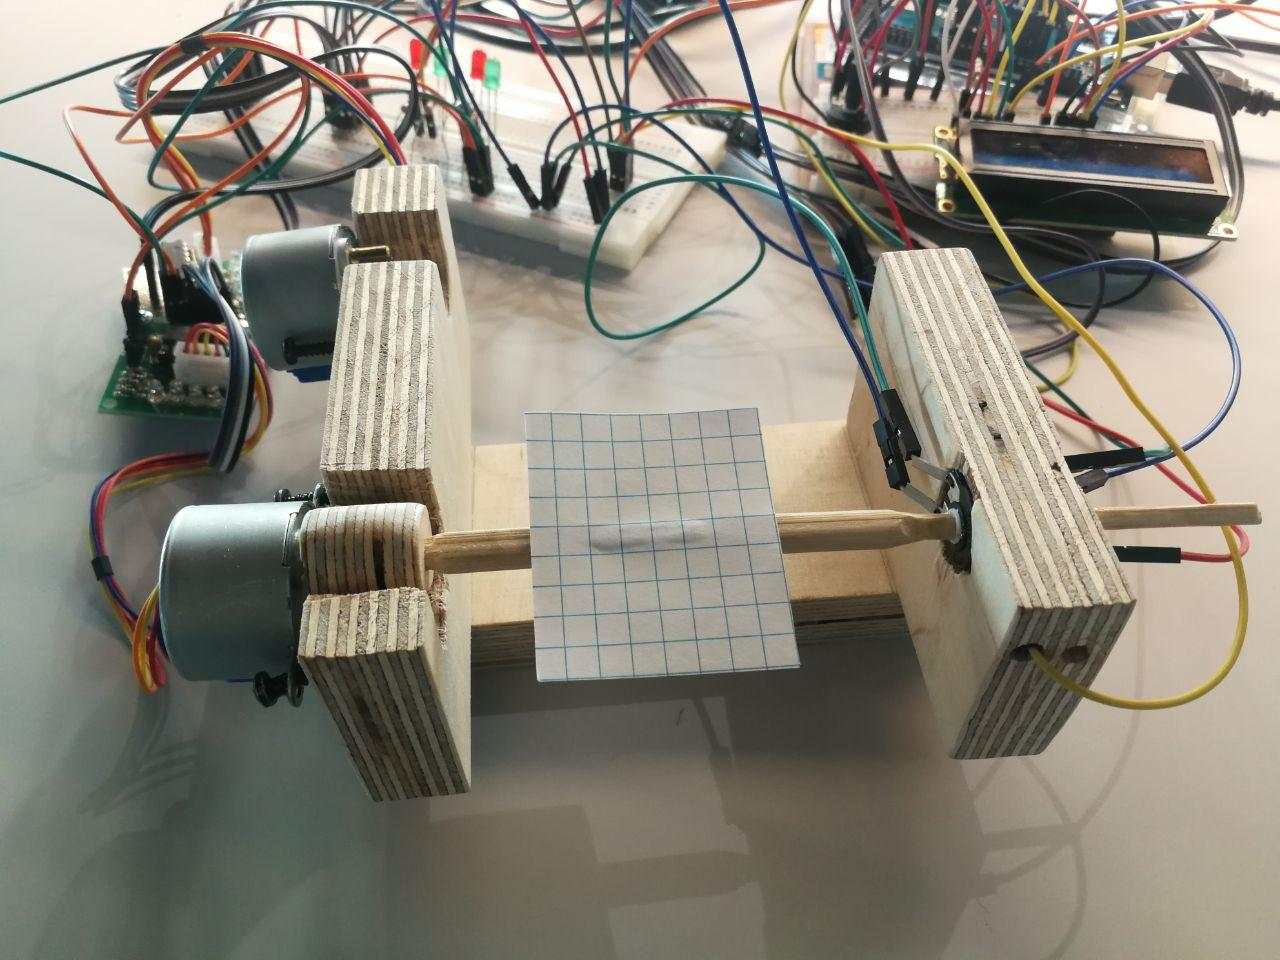
\includegraphics[width=\textwidth]{figures/mech01.jpg}
    \end{subfigure}
    \begin{subfigure}[b]{0.49\textwidth}
       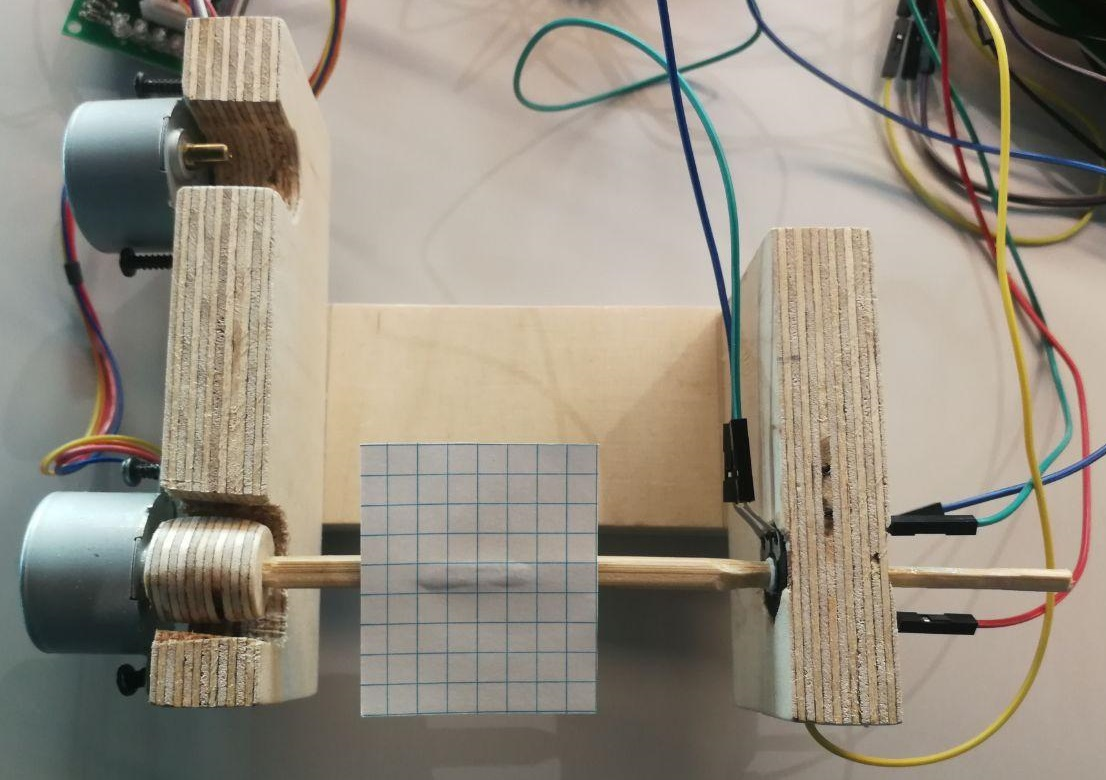
\includegraphics[width=\textwidth]{figures/mech02.jpg}
    \end{subfigure}
    \caption{Solar panel mounting structure}
    \label{fig:mech_design}
\end{figure}{}



